\documentclass[t]{beamer}

%%% Работа с русским языком
\usepackage{cmap}					% поиск в PDF
\usepackage{mathtext} 				% русские буквы в формулах
\usepackage[T2A]{fontenc}			% кодировка
\usepackage[utf8]{inputenc}			% кодировка исходного текста
\usepackage[english,russian]{babel}	% локализация и переносы

%% Beamer по-русски
\newtheorem{rtheorem}{Теорема}
\newtheorem{rproof}{Доказательство}
\newtheorem{rexample}{Пример}

%%% Дополнительная работа с математикой
\usepackage{amsmath,amsfonts,amssymb,amsthm,mathtools} % AMS
\usepackage{icomma} % "Умная" запятая: $0,2$ --- число, $0, 2$ --- перечисление

%%% Работа с картинками
\usepackage{graphicx}  % Для вставки рисунков
\graphicspath{{images/}{images2/}}  % папки с картинками
\setlength\fboxsep{3pt} % Отступ рамки \fbox{} от рисунка
\setlength\fboxrule{1pt} % Толщина линий рамки \fbox{}
\usepackage{wrapfig} % Обтекание рисунков текстом

%%% Работа с таблицами
\usepackage{array,tabularx,tabulary,booktabs} % Дополнительная работа с таблицами
\usepackage{longtable}  % Длинные таблицы
\usepackage{multirow} % Слияние строк в таблице

%%% Программирование
\usepackage{etoolbox} % логические операторы

%%% Другие пакеты
\usepackage{lastpage} % Узнать, сколько всего страниц в документе.
\usepackage{soul} % Модификаторы начертания
\usepackage{csquotes} % Еще инструменты для ссылок
%\usepackage[style=authoryear,maxcitenames=2,backend=biber,sorting=nty]{biblatex}
\usepackage{multicol} % Несколько колонок

%%% Картинки
\usepackage{tikz} % Работа с графикой
\usepackage{pgfplots}
\usepackage{pgfplotstable}

\usetheme{Frankfurt}

\title{Решение квадратных уравнений}
\author{А.~Н.~Золкин}
\date{\today}

\begin{document}
\frame[plain]{\titlepage}

\begin{frame}
    \frametitle{Сегодня в программе:}
    \tableofcontents
\end{frame}

\section{Введение}
\begin{frame}
    \frametitle{\insertsection}
    Человечеству известно множество методов решения квадратных уравнений.
    Самые известные из них:
    \begin{itemize}
        \item Общая формула вычисления корней
        \item Прямая и обратная теорема Виета
        \item Разложение квадратного трёхчлена на линейные множители
        \item Графическое решение
    \end{itemize} \pause
    Сегодня мы рассмотрим решение с помощью \textbf{общей формулы вычисления корней}
\end{frame}

\section{Общий вид}
\begin{frame}
    \frametitle{Общий вид уравнения}
    Квадратное уравнение в общем случае имеет вид
    \begin{center}
        $ax^2 + bx + c = 0$,
    \end{center}
    где $x$ -- неизвестное, $a, b, c$ -- коэффициенты, причём $a \neq 0$ \\
    \pause
    Рассматривать ход решения будем на примере:
    \begin{center}
        $3x^2 - 14x - 5 = 0$
    \end{center}
    \pause Предисловие окончено, \alert{\textbf{приступаем к алгоритму}}
\end{frame}

\section{Коэффициенты}
\begin{frame}
    \frametitle{Определение коэффициентов}
    \begin{tabular}{cl}
        \begin{tabular}{c}
            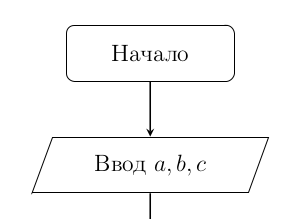
\includegraphics[scale=0.35]{Input.png}
        \end{tabular}
         & \begin{tabular}{l}
            \parbox{0.55\linewidth}{
                Коэффициенты определяют имеет ли квадратное уравнение решения на поле действительных чисел. \\
                \textbf{Поэтому их необходимо определить в первую очередь.}
            }
        \end{tabular} \\
    \end{tabular}
    Вернемся к нашему примеру и определим коэффициенты: \\ \pause
    \begin{itemize}
        \item $a=3$ \pause
        \item $b=-14$ \pause
        \item $c=-5$
    \end{itemize}
\end{frame}

\section{Дискриминант}
\begin{frame}
    \frametitle{Вычисление дискриминанта}
    \begin{tabular}{cl}
        \begin{tabular}{c}
            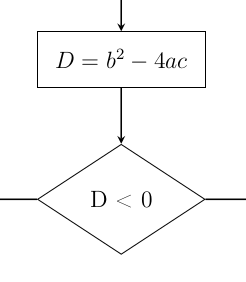
\includegraphics[scale=0.35]{CalcD.png}
        \end{tabular}
         & \begin{tabular}{l}
            \parbox{0.55\linewidth}{
                Дискриминант вычисляется по формуле показанной на рисунке слева.
                Знак дискримананта позволяет понять есть ли у уравнения действительные корни и количество таких корней.
            }
        \end{tabular} \\
    \end{tabular}
    Найдем дискриминант для нашего примера: \\ \pause
    \begin{center}
        $D = (-14)^2 - 4 \cdot 3 \cdot (-5) = 196 + 60 = 256$ \\
        $256 > 0 => D - положительный$
    \end{center}
\end{frame}

\section{$D < 0$}
\begin{frame}
    \frametitle{Отрицательный дискриминант}
    \begin{tabular}{cl}
        \begin{tabular}{c}
            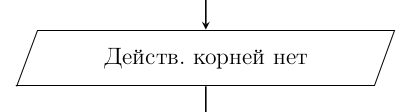
\includegraphics[scale=0.3]{SmallD.png}
        \end{tabular}
         & \begin{tabular}{l}
            \parbox{0.55\linewidth}{
                \alert{При отрицательном дискриминанте у уравнения отсутствуют действительные корни}
            }
        \end{tabular} \\
    \end{tabular}
\end{frame}

\section{Корни}
\begin{frame}
    \frametitle{Вычисление корней}
    \begin{tabular}{cl}
        \begin{tabular}{c}
            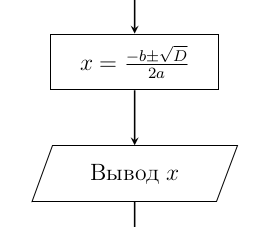
\includegraphics[scale=0.35]{BigD.png}
        \end{tabular}
         & \begin{tabular}{l}
            \parbox{0.55\linewidth}{
                Корни квадратного уравнения находятся по формуле представленной на рисунке слева.
            }
        \end{tabular} \\
    \end{tabular}
    Найдем корни для нашего примера: \\ \pause
    \begin{itemize}
        \item $x_1 = \frac{14+16}{6} = 5$
        \item $x_2 = \frac{14-16}{6} = -\frac{1}{3}$
    \end{itemize}
\end{frame}

\begin{frame}
    \begin{center}
        Спасибо за внимание!
    \end{center}
\end{frame}

\end{document}
